\documentclass[11pt,a4paper]{article}

\usepackage[T1]{fontenc}
\usepackage[utf8]{inputenc}
\usepackage{lmodern}
\usepackage[margin=1in]{geometry}
\usepackage{graphicx}
\usepackage{caption}
\usepackage{setspace}
\usepackage{parskip}

\setlength{\parindent}{0pt}
\setlength{\emergencystretch}{2em}
\setstretch{1.05}

\title{Hybrid Coarse-to-Fine Profilometry for Rough Surfaces: A Coincidence-Proxy Height-Fidelity Benchmark on Measured Surfaces}
\author{Dawid Kucharski\\
Division of Metrology and Measurement Systems, Institute of Mechanical Technology,\\
Faculty of Mechanical Engineering, Poznan University of Technology,\\
60-965 Poznan, Poland\\
\texttt{dawid.kucharski@put.poznan.pl}}
\date{}

\makeatletter
\renewcommand{\refname}{}
\makeatother

\begin{document}

\maketitle

Optical profilometry remains an important route for surface-topography evaluation in precision manufacturing and functional-surface metrology~\cite{vorburger1981}. Classical four-step phase-shifting interferometry (PSI) remains a strong practical baseline, and environmentally robust implementations are still an active issue in interferometric testing~\cite{mcdonnell2020}. Its estimation accuracy is also limited by phase-step and photon-statistical constraints~\cite{okamoto2021}. In parallel, quantum-entangled photon interferometry~\cite{richards2004} and high-visibility two-photon interference schemes~\cite{rarity1993} have motivated nonclassical sensing architectures. What remains unclear is whether such channels improve practically relevant rough-surface metrology endpoints under fair comparison conditions.

This paper presents a simulation benchmark of rough-surface profilometry comparing classical four-step phase-shifting interferometry (PSI), coincidence-proxy channels, and coarse-to-fine hybrid reconstruction under matched detected-count assumptions. The study uses 59 focus-variation (FV) topographies exported as Mountains/DigitalSurf \texttt{.sur} files as measured geometric references for simulated optical observations and is intended as a benchmark of reconstruction architectures rather than as a laboratory demonstration of quantum-enhanced metrology.

Figure~\ref{fig:rmse} summarises the main robust result, which is limited to height fidelity: on the measured-surface benchmark the hybrid branch gives the lowest surface-level median detrended height RMSE (314.0~nm), wins height RMSE on 32 of 59 surfaces, and remains below an optimistic classical-frontier oracle assembled from stronger auxiliary classical workflows (559.1~nm). Roughness-endpoint rankings are weaker and must be read cautiously. Figure~\ref{fig:roughness} shows the corresponding native-grid roughness comparison. A matched-bandwidth control shows that the apparent native-grid $S_q$ advantage of the direct coincidence-proxy branch is largely explained by reference-bandwidth mismatch, treatment holdouts reduce agreement to 50.0\% for $|\Delta S_a|$ and 0.0\% for $|\Delta S_q|$, and even the best native-grid $|\Delta S_z|$ branch exceeds the descriptor-scaled tolerance band on 74.6\% of surfaces. Classical two-colour and classical-frontier controls further show that envelope-following behaviour is not uniquely nonclassical.

A rate-based coincidence control sharpens the same conclusion: under ideal matched-count rates the hybrid branch remains best in height RMSE (290.9~nm), while under non-ideal detector assumptions the direct branch degrades to 1308.3~nm and the hybrid to 376.3~nm. The supported design rule is therefore architectural and narrow: within the present proxy benchmark, coincidence-derived information is most defensible as a coarse absolute-height prior inside a hybrid estimator when fixed-workflow height fidelity is the primary endpoint. Experimental validation remains necessary before stronger quantum-metrology claims can be made.

\textbf{Keywords:} coincidence-proxy interferometry; simulation benchmark; surface profilometry; hybrid reconstruction; coarse-to-fine reconstruction; phase-shifting interferometry; synthetic wavelength; roughness metrology; focus-variation microscopy; areal surface texture

\begin{figure}[htbp]
    \centering
    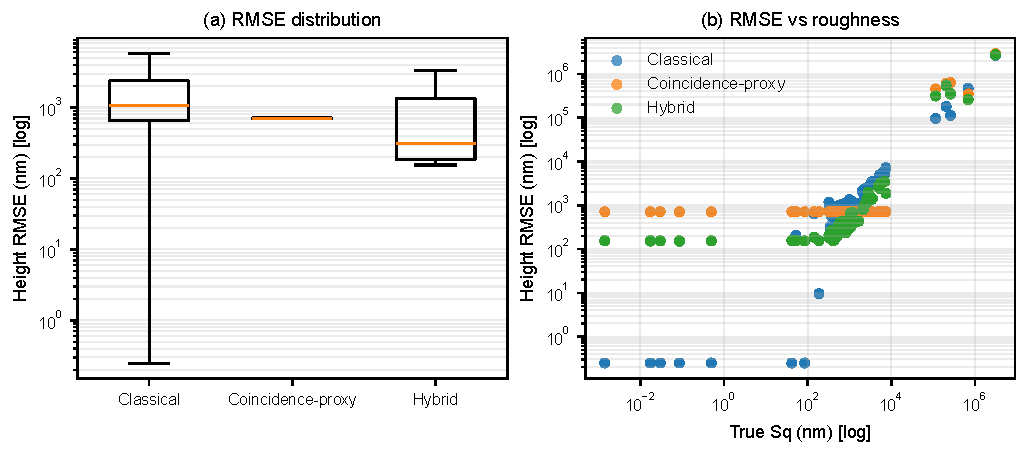
\includegraphics[width=0.92\textwidth]{../outputs/paper_alicona_benchmark/figures/rmse_measured_summary.pdf}
    \caption{Measured-surface benchmark summary across all FV \texttt{.sur} samples: height RMSE distributions by method and RMSE trends vs surface roughness. All values are computed from the measured height maps (after plane detrending).}
    \label{fig:rmse}
\end{figure}

\begin{figure}[htbp]
    \centering
    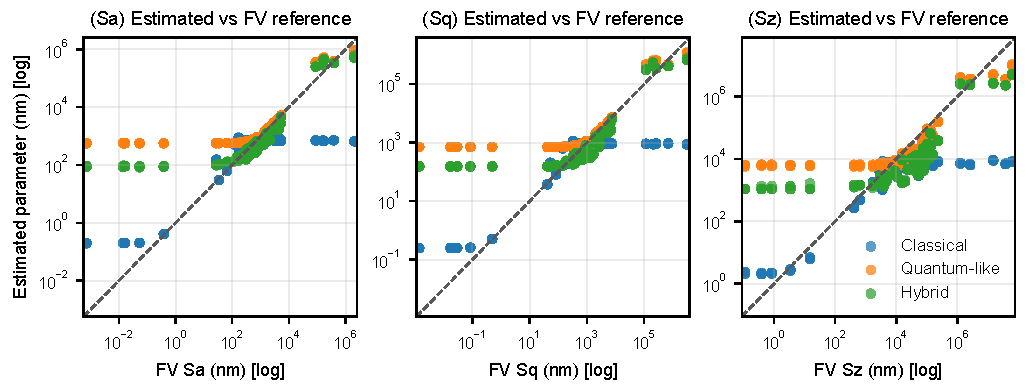
\includegraphics[width=0.92\textwidth]{../outputs/paper_alicona_benchmark/figures/roughness_measured_summary.pdf}
    \caption{Direct comparison of areal roughness parameters estimated from the simulated interferometric reconstructions against the corresponding values computed from the Alicona reference height maps. Each point is one measured \texttt{.sur} surface; the dashed line marks perfect agreement. This native-grid view is diagnostic rather than definitive for workflow selection because the interferometric forward model operates on the downsampled benchmark grid. The hybrid branch remains strongest for $S_a$, whereas the direct coincidence-proxy branch more often follows the native-grid $S_q$ and $S_z$ values because it retains broad-envelope excursions more readily than fine texture.}
    \label{fig:roughness}
\end{figure}

\bigskip
\noindent\textbf{References}

\begin{thebibliography}{99}

\bibitem{vorburger1981}
T. V. Vorburger and E. C. Teague,
``Optical techniques for on-line measurement of surface topography,''
\emph{Precision Engineering}, vol. 3, pp. 61--83, 1981.

\bibitem{mcdonnell2020}
E. M. McDonnell and L. L. Deck,
``Solutions for environmentally robust interferometric optical testing,''
in \emph{Proceedings of SPIE}, vol. 11487, 2020.

\bibitem{okamoto2021}
R. Okamoto and T. Tahara,
``Precision limit for simultaneous phase and transmittance estimation with phase-shifting interferometry,''
\emph{Physical Review A}, vol. 104, 033521, 2021.

\bibitem{richards2004}
R. K. Richards,
``Quantum-entangled photon interferometry,''
in \emph{Interf. XII: Tech. Anal.}, vol. 5531, pp. 17--23, 2004.

\bibitem{rarity1993}
J. G. Rarity, J. Burnett, P. R. Tapster, and R. Paschotta,
``High-visibility two-photon interference in a single-mode-fibre interferometer,''
\emph{EPL}, vol. 22, pp. 95--100, 1993.

\end{thebibliography}

\end{document}